\documentclass[12pt]{article}
\usepackage{graphicx}
\usepackage{amsmath}

\usepackage[margin=1in]{geometry}
\usepackage{float}
\usepackage{listings}
\usepackage{booktabs}

\title{Labwork 5: Gaussian Blur Convolution}
\author{Ngo Quang Truong 2540106}
\date{3 Oct 2026}

\begin{document}

\maketitle
\newpage

\section{Introduction}

This report presents an implementation of a $7\times7$ Gaussian blur filter on an RGB image, using three approaches: a sequential CPU implementation, a CUDA GPU implementation that reads directly from global memory, and a CUDA GPU implementation that uses shared memory.

\section{Method}
A Gaussian blur is a convolution between the image and a 2D kernel that follows a normal distribution:
\begin{equation}
G(x,y) = \frac{1}{2\pi\sigma^2}\exp\left[-\frac{(x-\mu_x)^2+(y-\mu_y)^2}{2\sigma^2}\right]
\end{equation}

The discrete, normalized $7\times7$ kernel used in this labwork is:
\[
\frac{1}{1003}
\begin{bmatrix}
0 & 0 & 1 & 2 & 1 & 0 & 0\\
0 & 3 & 13 & 22 & 13 & 3 & 0\\
1 & 13 & 59 & 97 & 59 & 13 & 1\\
2 & 22 & 97 & 159 & 97 & 22 & 2\\
1 & 13 & 59 & 97 & 59 & 13 & 1\\
0 & 3 & 13 & 22 & 13 & 3 & 0\\
0 & 0 & 1 & 2 & 1 & 0 & 0
\end{bmatrix}
\]
For every output pixel, each color channel is replaced by the weighted sum of its $7\times7$ neighborhood with this kernel. Pixels outside the image border are handled with zero/edge padding (pad $=3$ on every side, since $\lfloor 7/2 \rfloor = 3$).

Test image: a $1920\times1080$ RGB image.

\begin{figure}[h]
    \centering
    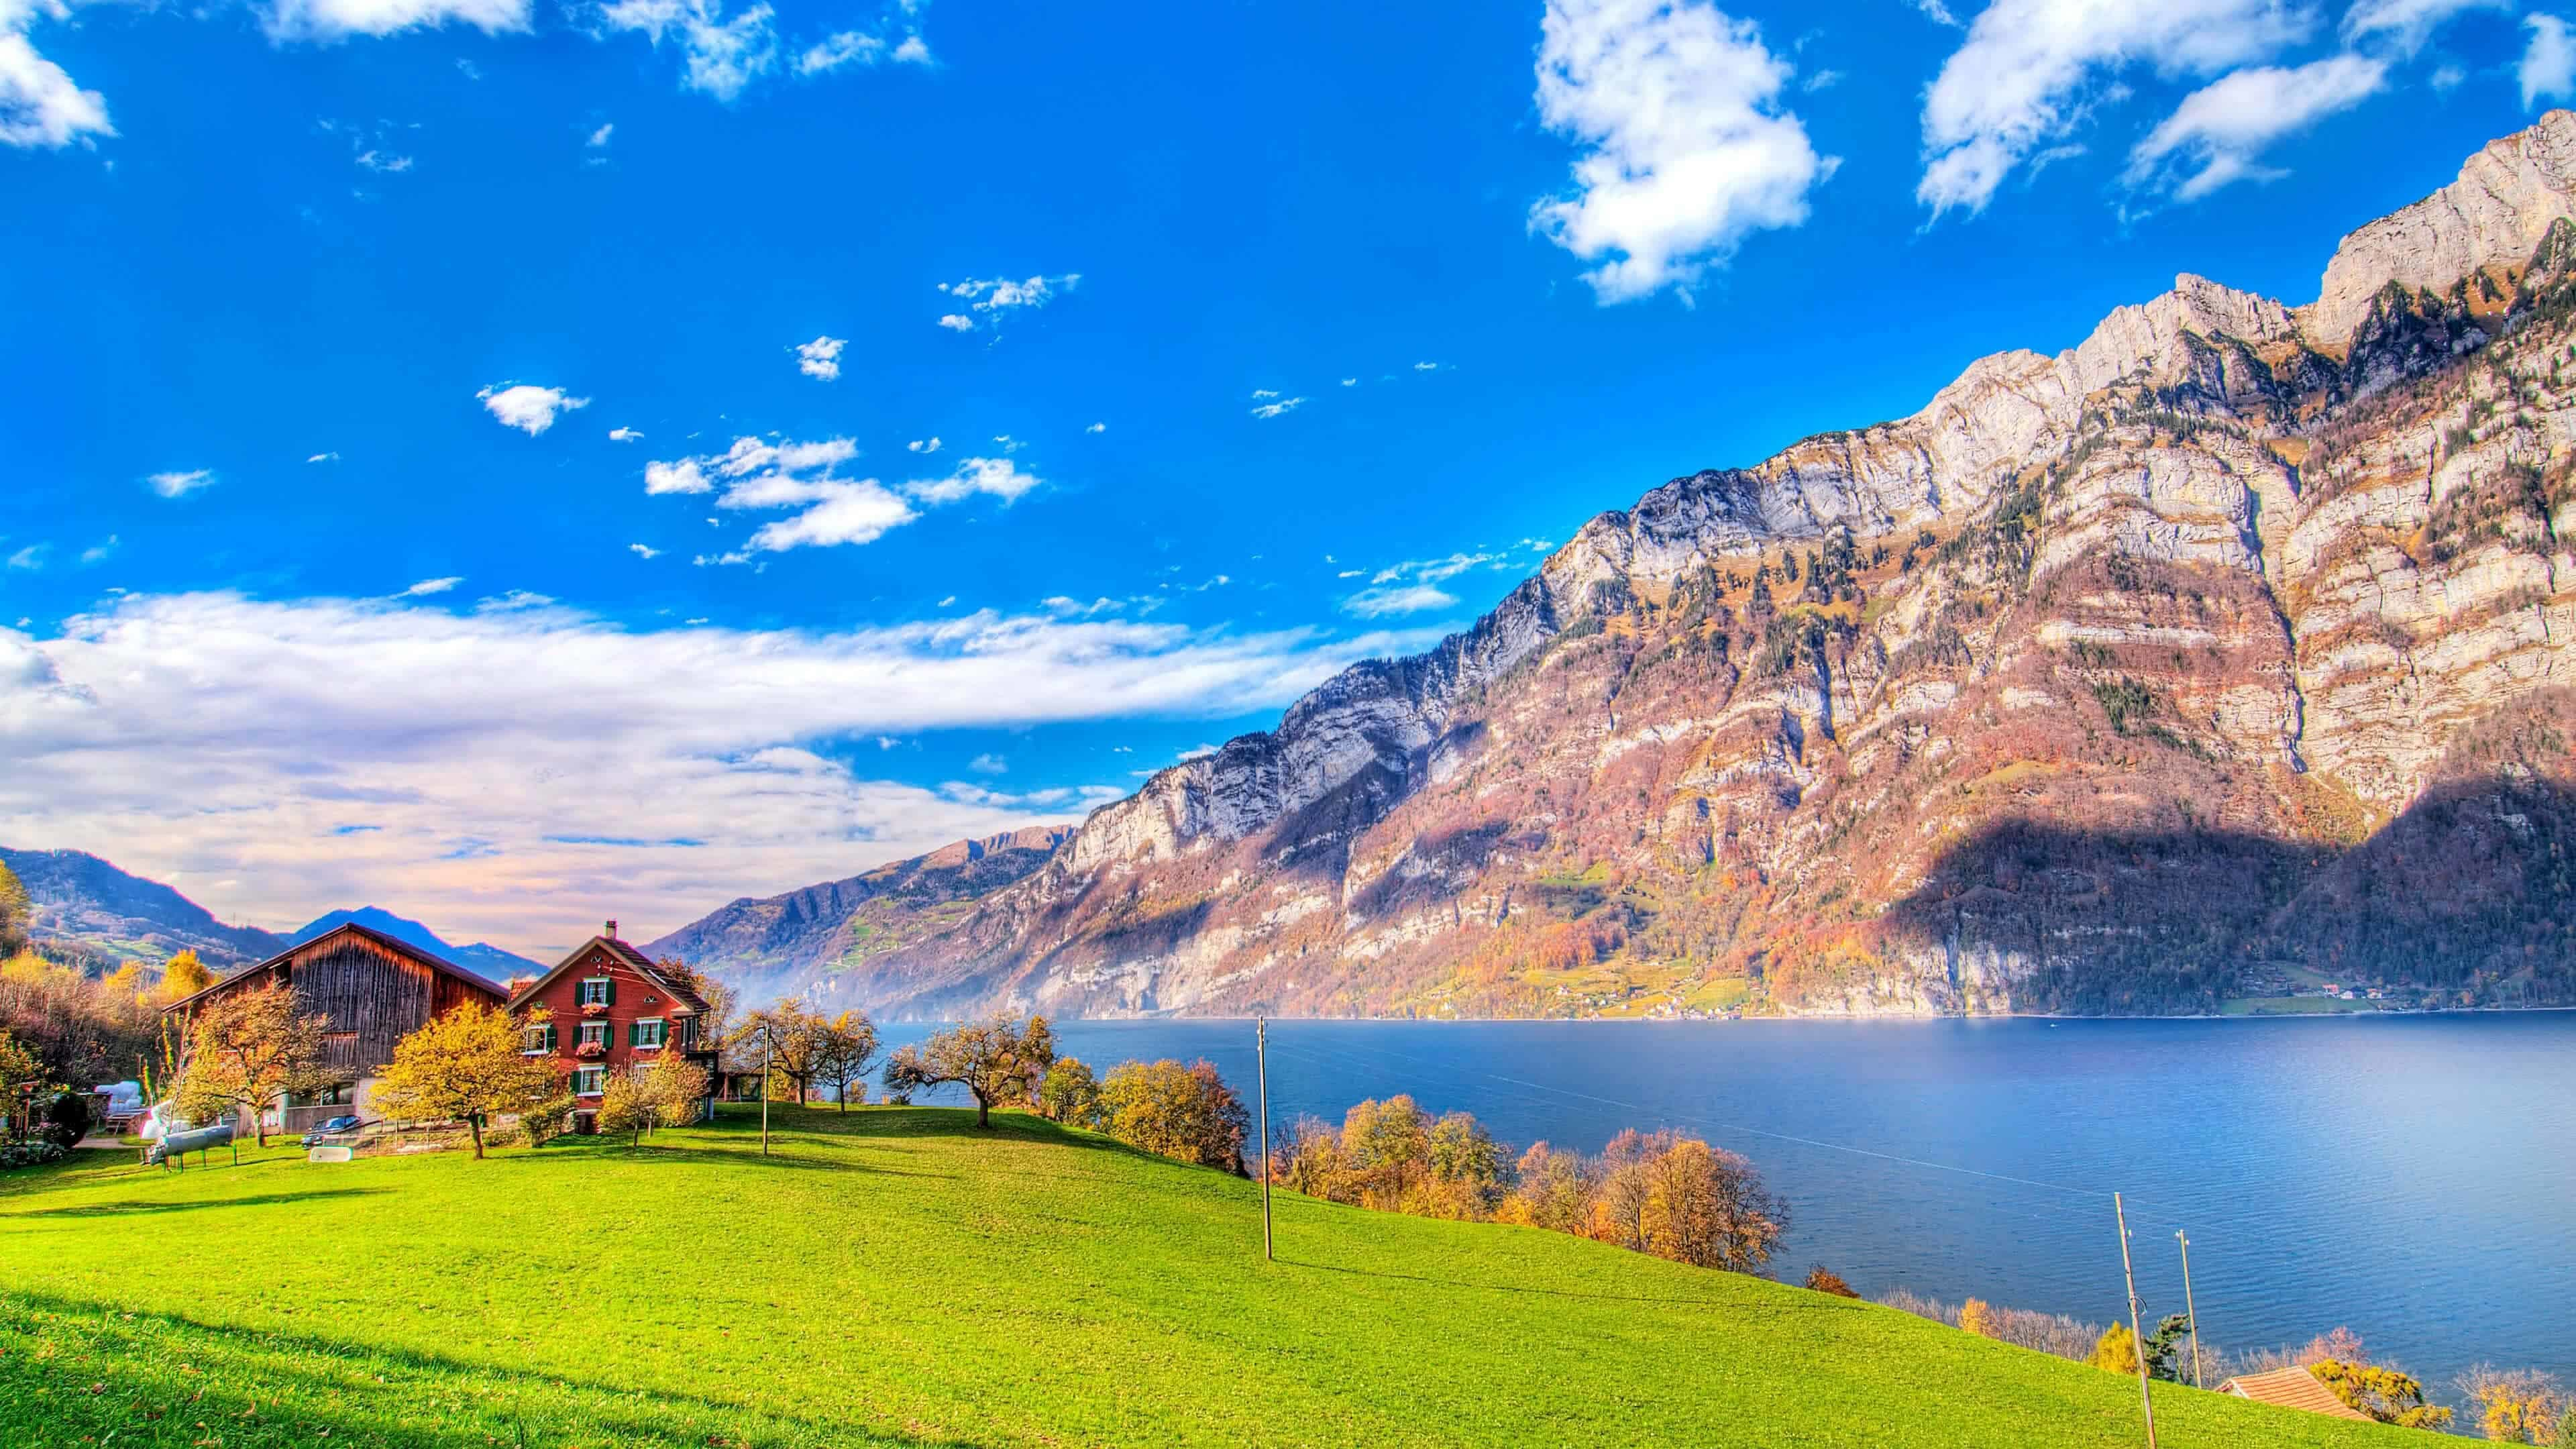
\includegraphics[width=0.5\textwidth]{original_image.jpg}
    \caption{Original RGB image}
    \label{fig:original_image}
\end{figure}

\section{CPU Implementation}
The CPU version pads the image, then loops over every pixel, every channel, and every kernel weight sequentially (three nested loops plus the $7\times7$ convolution window).

\begin{figure}[H]
    \centering
    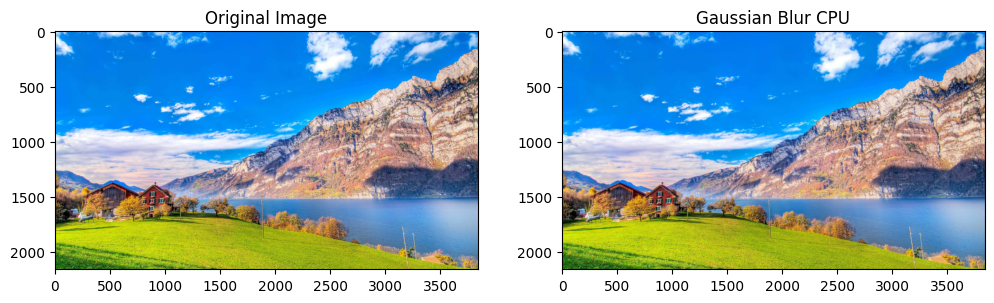
\includegraphics[width=0.9\textwidth]{CPU_Output.png}
    \caption{CPU Gaussian blur output}
    \label{fig:cpu_output}
\end{figure}

\section{GPU Implementation without Shared Memory}
Each CUDA thread is assigned one output pixel through \texttt{cuda.grid(2)}. The thread independently reads its own $7\times7$ neighborhood directly from global memory, multiplies by the kernel, and writes the result back.
\begin{figure}[H]
    \centering
    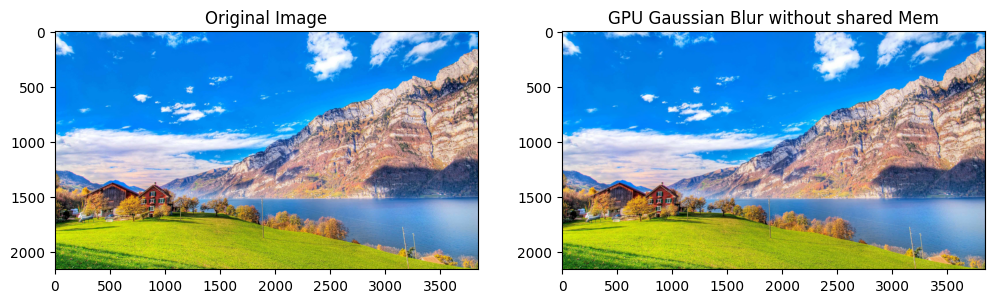
\includegraphics[width=0.9\textwidth]{GPU_Output_NoShared.png}
    \caption{GPU Gaussian blur output (no shared memory)}
    \label{fig:gpu_noshared_output}
\end{figure}

\section{GPU Implementation with Shared Memory}
To reduce redundant global memory traffic, this version has every block cooperatively load its pixels into a shared memory tile of size $(16+2\times3)\times(16+2\times3) = 22\times22$ before any computation happens. A \texttt{cuda.syncthreads()} barrier ensures the tile is fully populated before any thread starts reading from it.

\begin{figure}[H]
    \centering
    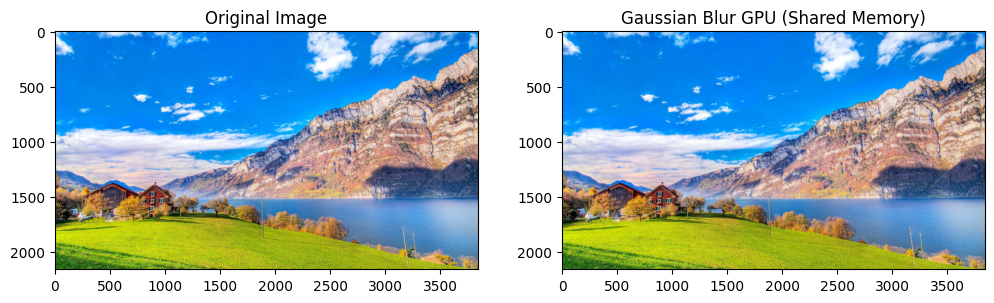
\includegraphics[width=0.9\textwidth]{GPU_Output_Shared.png}
    \caption{GPU Gaussian blur output (shared memory)}
    \label{fig:gpu_shared_output}
\end{figure}

\section{Results}

\begin{table}[H]
\centering
\begin{tabular}{lcc}
\toprule
Implementation & Time (s) & Speedup vs CPU \\
\midrule
CPU (sequential) & 174.747945 & $1\times$ \\
GPU, no shared memory & 0.713428 & $\approx 245\times$ \\
GPU, shared memory & 0.4778 & $\approx 366\times$ \\
\bottomrule
\end{tabular}
\caption{Execution time and speedup for the $7\times7$ Gaussian blur, $16\times16$ thread block.}
\label{tab:results}
\end{table}

Using shared memory further reduces the runtime from 0.713 s to 0.478 s, an additional $\approx 1.49\times$ speedup over the GPU version without shared memory.

\end{document}
